% !Mode:: "TeX:UTF-8"
% !TEX program  = xelatex
\documentclass[a4paper]{article}
\usepackage{amsmath}
\usepackage{amssymb}
\usepackage{ctex}
\usepackage{braket}
%\usepackage[european]{circuitikz}
\usepackage{multirow}
\usepackage{float}
\usepackage{colortbl}
\usepackage{graphicx}
\usepackage{geometry}
\geometry{left=2.5cm,right=2.5cm,bottom=2.5cm,top=2.5cm}

\usepackage{physics}
\usepackage{mhchem}
\usepackage{siunitx}
\usepackage{bm}
\DeclareMathOperator{\e}{\mathrm{e}}
\DeclareMathOperator{\I}{\mathrm{i}}


\title{近代物理实验报告:单电子固态量子计算}
\author{\quad 学号\quad 匡亚明学院}
\date{2019年2月29日}
\begin{document}
\maketitle
\bibliographystyle{unsrt}

\tableofcontents
\newpage
%--------main-body------------

\section{引言}


%\section{实验目的}
\subsection{量子计算背景}
过去的几十年中,经典计算机经历了快速的发展时期。第一台通用电子计算机ENIAC
占地约170平方米,如今的掌上电脑已经可以放进口袋。体积的巨大变化,主要归功
于集成电路工业的飞速发展。英特尔公司创始人之一戈登·摩尔曾提出著名的摩尔定
律,用以总结和预期集成电路的发展,即集成电路上可容纳的晶体管数目,约每隔18
个月便会翻一倍,其性能也会翻倍。然而随着电路集成度越来越高,摩尔定律也遇到
了新的挑战。因为按照摩尔定律描述的发展趋势,集成电路的工艺己进入纳米尺度。
在芯片上如此高密度的集成元器件,热耗散问题是一个巨大的挑战。更严重的是,随
着集成电路的工艺进入纳米尺度,量子效应会逐渐显现并占据支配地位。当描述元器
件工作的物理规律由经典物理转变为量子力学,试图按照原来的方式保持集成电路的
发展趋势就非常困难了。

既然在微观尺度下,量子力学效应占主导,那有没有可能利用量子力学效应来构
造计算机呢?费曼最先在1982年指出,采用经典计算机不可能以有效方式来模拟量子
系统的演化。我们知道,经典计算机与量子系统遵从不同的物理规律,用于描述量子
态演化所需要的经典信息量,远远大于用来以同样精度描述相应的经典系统所需的经
典信息量。费曼提出用量子计算则可以精确而方便地实现这种模拟。1985 年,David
Deutsch深入研究了量子计算机是否比经典计算机更有效率的问题。他首次在理论上
描述出了量子计算机的简单模型——量子图灵机模型,研究了它的一般性质,预言了
它的潜在能力。但当时的人们还不知道有什么具体的可求解问题,量子计算能比经典
计算更有优越性。1994年,美国数学家Peter Shor从原理上指出,量子计算机可以用
比经典计算机快得多的速度来求解大数的质因子分解问题。由于大数质因子分解问题
是现代通信与信息安全的基石,Shor的开创性工作引起了巨大的关注,其可期待的辉
煌应用潜力有力地刺激了量子计算机和量子密码等领域的研究发展,成为量子信息科
学发展的重要里程碑之一。1996 年Grover发现了另一种很有用的量子算法,即所谓
的量子搜索算法,它适用于解决如下问题: 从$ N $个未分类的客体中寻找出某个特定的
客体。经典算法只能是一个接一个地搜寻,直到找到所要的客体为止,这种算法平均
地讲要寻找$ N/2 $次,成功几率为$ 1/2 $,而采用Grover的量子算法则只需要
$ \sqrt{N} $次。

随着一系列量子算法的提出,量子计算对某些重要问题相对于己知的经典计算方
式的计算能力的展现出巨大的优势。量子计算不仅吸引着众多的科研人员,其应用前
景也吸引了谷歌、微软、IBM 等国际知名公司参与这一领域的竞争。近年来,各研究团队更是试图实现“量子霸权”(Quantum supremacy),即通过量子计算实现对经典计算能力的极限的突破

\section{实验原理}
\subsection{量子计算基本概念}
经典计算机需要信息的载体,逻辑操作,状态读出等一系列基本元素。量子计算机也
类似,首先我们需要量子信息的载体,即量子比特。然后需要具备对量子比特进行初
始化,操控和读出的能力。我们利用一系列的逻辑操作,构成量子算法,来实现特定
的计算目的。
\subsubsection{量子比特}
\begin{figure}[H]
	\centering
	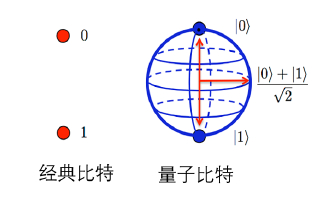
\includegraphics[width=0.4\linewidth]{fig/1.jpg}
	\caption{经典比特与量子比特对比示意图}
\end{figure}
如果我们把数据送入计算机处理,就必须把数据表示成为计算机能识别的形式。
在经典计算机中,信息单元用1个二进制位表示,它处于“0”态或“1”态。而在量子
计算机中,信息单元称为“量子比特”,它除了可以处于“0”态或“1”态外,还可处
于一种叠加态。我们用$ \ket{0} $和$ \ket{1} $表示量子比特可取的状态基失,单个量子比特可取的为
\begin{equation}\label{key}
\ket{Psi} = \alpha\ket{0} + \beta\ket{1}
\end{equation}
由于$ \alpha^*\alpha + \beta^*\beta = 1 $,们也可以这样表示量子比特:
\begin{equation}\label{key}
\ket{\Psi} = \cos\dfrac{\theta}{2}\ket{0} + \e^{\I\phi}\sin\dfrac{\theta}{2}\ket{1}
\end{equation}
其中$ -\pi \leq \theta \leq \pi, 0\leq \phi \leq 2\pi $. 显然$ \theta $和
$ \phi $在单位三维球体上定义了一个点,这个球体通常被称为布洛赫球。单个量子比特的
纯态可以与布洛赫球面上的点一一对应.

\subsubsection{量子逻辑门}
经典计算中用到很多基本逻辑门,包括与门、或门、非门、异或门、与非门和或非门
等,这些元件组合在一起能构成用来计算任何函数的硬件电路。量子计算机与此类
似,也由一系列的量子门组合而成,以此来完成复杂计算任务。图\ref{fig:gate}列出了常用的量子逻辑门,其代表符号和矩阵表示。描述单个量子门的矩阵$ U $要求必须是幺正的,
即$ U U^\dagger = I $. C-NOT门是一个两比特门,当控制比特是$ \ket{0} $时,目标比特不变。当控制比特是$ \ket{1} $时,目标比特发生翻转。\\
\begin{figure}[H]
	\centering
	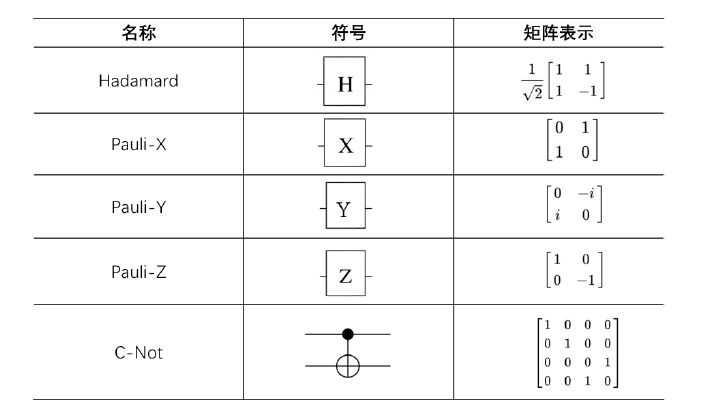
\includegraphics[width=0.8\linewidth]{fig/2.jpg}
	\caption{常用量子逻辑门的符号和矩阵表示}
	\label{fig:gate}
\end{figure}
要实现实用的量子计算,需要的量子比特的数目远不止两个,因此需要能够实现多比特的量子逻辑门。而且,量子计算中需要施加的量子逻辑门与要解决的问题有关,也就是说,为了解决不同的问题,需要使用不同的量子逻辑门。那么,能不能只用一些基本的量子逻辑门,来实现任意的量子逻辑门的效果呢? 理论上可以证明,对于任意的多比特量子逻辑门,都可以通过两比特受控非门结合单比特量子逻辑门的方式实现。我们称单比特量子逻辑门和受控非门形成一组普适的量子逻辑门。

\subsubsection{量子测量}
为了得到量子计算的结果,需要对末态进行量子测量。对于量子比特$ \ket{\Psi} = \alpha\ket{0} + \beta\ket{1} $,采用基矢$ \ket{0} $,$ \ket{1} $进行测量,得到结果$ \ket{0} $和$ \ket{1} $的几率分别为$ \abs{\alpha}^2 $和$ \abs{\beta}^2 $。如
果选择另外的一组正交基矢:
\begin{equation}\label{key}
\ket{+} = \dfrac{1}{\sqrt{2}}(\ket{0} + \ket{1})  \qquad \ket{-} = \dfrac{1}{\sqrt{2}}(\ket{0} - \ket{1})
\end{equation}
任意量子比特的态可以写成:
\begin{equation}\label{key}
\ket{\Psi} = \alpha\ket{0} + \beta\ket{1} = \dfrac{\alpha+\beta}{\sqrt{2}}\ket{+} + \dfrac{\alpha-\beta}{\sqrt{2}}\ket{-}
\end{equation}
测量之后,坍缩到$ \ket{+} $或者$ \ket{-} $的几率分别为$ \abs{\alpha+\beta}^2/2 $,$ \abs{\alpha-\beta}^2/2 $.\\
一般情况下,给出任意的基矢$ \ket{a} $和$ \ket{b} $,可以将任意态表示为$ \alpha\ket{a}+ \beta\ket{b} $,只要$ \ket{a} $和$ \ket{b} $是正交的,就可以进行相对于$ \ket{a} $和$ \ket{b} $的测量,以$ \abs{\alpha}^2 $的几率得到$ \ket{a} $,以$ \abs{\beta}^2 $的几率得到$ \ket{b} $。
\subsubsection{量子算法}
经典计算机在处理某些问题的时候,速度是很快的,比如计算乘法$ 127\cross 229 = \text{?} $。但如果将这个问题反过来,求解29083这个数能分解成哪两个质数是乘积$ \text{?}\cross\text{?} = 29083 $,这时候经典计算机可能要花费很长的时间来处理。尤其是当要分解的数非常大的时候,普通计算可能要运算几年或者更长的时间才能得到结果。而此时如果采用量子算法,则大数质因子分解问题可以迎刃而解。利用量子计算机,几乎可以瞬间完成大数分解。\\
量子算法与经典算法相比,其差别在于,量子算法融入了量子力学的很多特征。
经典算法本质上不依赖于量子物理,只是数学上的技巧。而量子算法中用到了量子相
干性、量子叠加性、量子并行性、波函数坍缩等量子力学特性,进而大大提高了来计
算效率。这种崭新的计算模式,给计算科学带来重大影响。有些问题,依据经典计算
复杂性理论,是不存在有效算法的,但在量子算法的框架里却找到了有效法。最为典
型的量子算法有:Shor算法(质因数分解),QEA算法(组合优化求解),Grover算法
(量子搜索算法)等。这些量子算法可能处理的问题不同,但是都是采用了量子力学
物理性质进行计算。每一种算法都有其独特性,比如Shor算法对质因素分解将直接
威胁RSA加密体系,Grover算法在搜索方面,指数级的加速。这些都有潜在的应用价
值。下面我们以Deutsch-Jozsa算法为例,说明量子并行性的优势。\\
\paragraph{Deutsch-Jozsa算法}~\\



\subsection{量子计算的实验实现}





\section{实验内容及结果}
\subsection{连续波实验}
\subsection{拉比振荡实验}
\subsection{$ T_2 $实验}
\subsection{D-J算法实验}
\subsection{设计实验}




%\section{实验数据}


\section{思考题}
\subsection*{请利用布洛赫球表示以下量子态:}

\subsection*{如果实验中施加的微波频率$ f $与共振频率$ f_0 $有偏差,即$ f = f_0 + \delta f $,拉比振荡的频率会如何变化?}

\subsection*{拉比振荡频率与微波功率的关系是什么?}

\subsection*{参照$ n=1 $的特殊情况,即图1.5所示的量子线路图,画出一般情况的D-J算法量子线路图,并解释算法原理}


%\nocite{jiaocai}
\bibliography{ref}
\end{document}